\documentclass[a4paper,11pt]{article}
%\documentclass[a4wide]{scrreprt}

%\usepackage{palatino}
\usepackage{hyperref}
\usepackage{graphicx}
\usepackage{array} 
\topmargin -1.5cm 
\oddsidemargin -0.04cm 
\evensidemargin -0.04cm 
\textwidth 16.59cm
\textheight 21.94cm

\parskip 7.2pt % sets spacing between paragraphs

%\renewcommand{\baselinestretch}{1.5} % Uncomment for 1.5 spacing between lines

\parindent 0pt % sets leading space for paragraphs

\title {Project Report \\ Kinect Controlled Robotic Arm \\ Group 10}
\author {Aayush Singhal\\09005041 \and Sivakanth Gopi\\09005043  \and Sriram Bhargav\\09005067 \and Aakash N S\\09005069}
\begin{document}
\maketitle

\begin{center}
\begin{large}
under the guidance of\\
\textbf{Prof. Kavi Arya}\\
\end{large}
\end{center}
\begin{center}

\includegraphics[scale=0.32]{images/iitb.png}
\end{center}
\begin{center}
\begin{large}
Embedded and Real-Time Systems Laboratory \\
Department of Computer Science and Engineering \\
Indian Institute of Technology \\
Bombay \\
\end{large}
\end{center}
%\pagenumbering{roman} % Roman page number for toc
%\setcounter{page}{1} % Make it start with "ii"

\newpage
\tableofcontents
\newpage

\begin{abstract}
The project aims at developing an simple and intuitive Natural User Interface (NUI) for controlling a robotic arm, using a human arm. All the user needs to do is stand in front of a sensor and move his arm, and the robotic arm tries to imitate the actions and movements of the human arm. As a result, fluid movements which cannot be performed using a controller, are now possible to execute. 

The Microsoft Kinect sensor is used to capture skeletal data of the user which is processed and converted into a set of angles which is then sent to the robotic arm over a serial port correction. The algorithm used to generate the angles tries to reach the same position in space as that of the human hand with respect to the human body, relative to the base of the robotic arm. This makes the control fairly intuitive even for first time users.

\end{abstract}

\section{Introduction}

Controlling a robotic arm with a traditional controller can be very difficult. It is non-intuitive, complex, and requires training to control the arm properly. It is difficult to control various degrees of freedom simultaneously, and thus the arm cannot be used to perform fluid movements that a human arm is capable of. Therefore, its full power cannot be realized using a traditional controller. 

There is a need for a Natural User Interface (NUI) using which a human arm can directly control a robotic arm. Such an interface would make the control the intuitive and easy. No special training would be required to control the arm and even first time users would find it easy to adjust to the controls. The arm can be deployed in remote or hostile places to perform actions and movements that would otherwise be impossible to perform. Robotic arms of various shapes and sizes, suited to various domains, can be controlled easily. The interface, therefore, would open up a plethora of applications.
\newpage

\section{Definitions}



\begin{table}[h]
\setlength{\tabcolsep}{10pt}
%\centering
\noindent\makebox[\textwidth]{
\begin{tabular}{|m{0.26\textwidth}|m{0.64\textwidth}|}
\hline
\textbf{Term}& \textbf{Definition} \\
\hline
Robotic Arm & A programmable mechanical arm wih similar functions to a human arm\\
\hline
Arm & Unless specified otherwise, refers to the robotic arm \\
\hline
Kinect & A motion sensing input device developed by Microsoft\\
\hline
User & The person controlling the robotic arm\\
\hline
Depth Data & The data produced by the depth image camera in Kinect. Each frame in the stream contains the distance, in mm, to the nearest object at each x and y coordinate in the camera's field of view.\\
\hline
Skeletal Data & The data provided by Kinect about the configuration of a skeleton, as a set of positions that compose the sleleton. The skeleton represents the user's position and posture.\\
\hline
VGA & Video Graphics Accelerator \\
\hline
SDK & Software Development Kit \\
\hline
IDE & Integrated Development Environment \\
\hline
API & Application Programming Interface \\
\hline
GUI & Graphical User Interface \\
\hline 
DirectX & A collection of API for handling multimedia related tasks, on Microsoft platforms \\
\hline
Microsoft Visual Studio & IDE for C\# programming for the robotic arm and Microsoft Kinect \\
\hline

\end{tabular}}
\end{table}
\newpage

\section{Hardware Architecture}
\begin{itemize}
\item The Microsoft Kinect Sensor is used to catpure depth data. The sensor is connected to a controller (running Windows 7, or Windows Embedded Standard 7, with the Microsoft Kinect SDK v1 and .NET Framework 4.0 or higher installed), where the depth data is processed to obtain skeletal tarcking data of the user. 

\begin{figure}[htp]
\centering
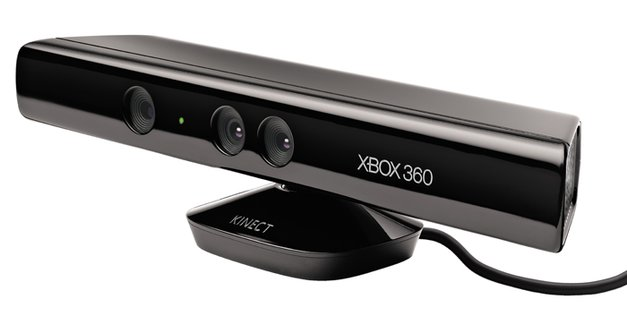
\includegraphics[scale=0.4]{images/kinect.jpg}
\caption{Microsoft Kinect} 
\end{figure}

\item The Dexter ER2 Heavy Duty Robotic Arm is used as the target arm. It has six degrees of freedom as shown in Figure 2. It has a maximum payload limit of 50 grams. The arm is controlled in real time by sending data from the controller, containing angles of ratations and rotation velocities of the axes, over a serial port.
\begin{figure}[htp]
\centering
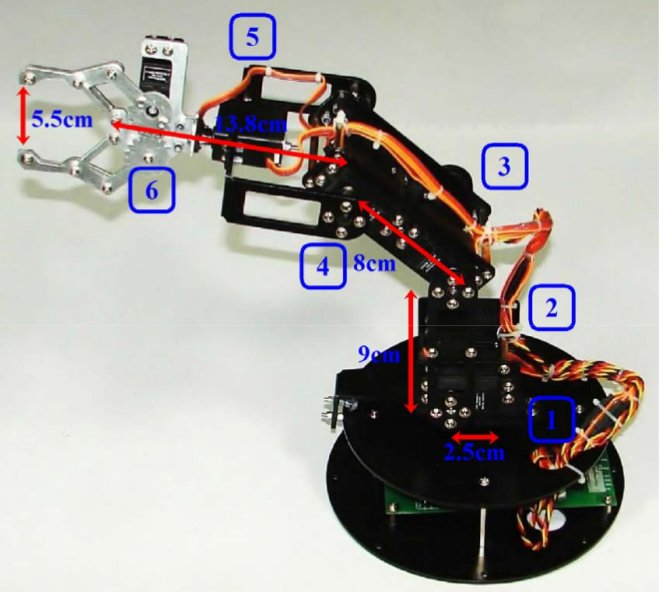
\includegraphics[scale=0.42]{images/arm-axes.jpg}
\caption{Dexter ER2 Heavy Duty Robotic Arm} 
\end{figure}

\begin{figure}[htp]
\centering
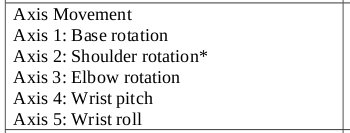
\includegraphics[scale=0.6]{images/arm-axes-table.jpg}
\caption{Axis Mappings of Dexter}
\end{figure}
\newpage
\end{itemize}

\section{Software Architecture}
The application consists of two modules : Main module, and 
\begin{enumerate}
\item \emph{API for Robotic Arm Control} : This module provides functions for controlling the Robotic Arm in real time over serial port. The .dll file can be used to control the robotic arm from any C\# project. Documentation for the library has been provided.
\item \emph{Main Module} : This module uses the above module to control the robotic arm. It provides a GUI for the application. Wrappers for accessing skeletal data obtained from Kinect and using the Two Circle Algorithm have been provided. These can be used from any C\# project. Documentation for the module has been provided.
\end{enumerate}

\begin{figure}[htp]
\centerline{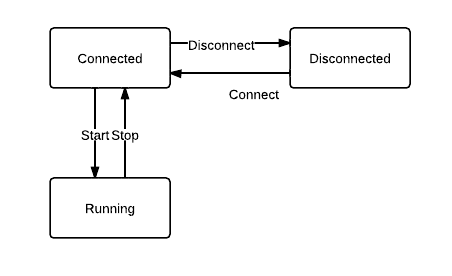
\includegraphics[scale=0.7]{images/guifsm.png}}
\caption{FSM for the Controller}\label{fig:exp}
\end{figure}

\newpage
\section{Work Division}
\begin{table}[h]
\setlength{\tabcolsep}{10pt}
%\centering
\noindent\makebox[\textwidth]{
\begin{tabular}{|m{0.4\textwidth}|m{0.25\textwidth}|}
\hline
\textbf{Work/Critical Tasks}& \textbf{People Responsible} \\
\hline
Module for Real Time Serial Port Communication with the arm& Aakash, Gopi, Bhargav\\
\hline
Module for Handling Sekletal Data and Performing Calculations & Aayush, Gopi, Bhargav\\
\hline
Design and Coding of the Two-Circle Algorithm & Gopi, Aayush, Aakash\\
\hline
Graphical User Interface (GUI) for the Application & Bhargav, Aayush, Gopi\\
\hline
Documentation & All\\
\hline
\end{tabular}}
\end{table}







\section{Innovations, Challenges and Solutions}
\subsection{Innovations and Challenges}
\begin{itemize}
\item Developing an API for controlling the robotic arm. 
\item Designing an intuitive control mechanism for the user.
\item Developing an algorithm for calculating the angles as a continuous function of the positoion of the human arm.
\item Implementing averaging features to remove deviations in the skeletal data obtained from Kinect.
\end{itemize}

\subsection{Problems and Solutions}
\begin{itemize}
\item API/Hardware manual for robotic arm was not available.
\begin{itemize}
\item decompiled the robotic arm control GUI, read and understood the code and developed an C\# API/library which future projects can use.
\end{itemize}
\item Kinect cannot capture finger and wrist movements
\begin{itemize}
\item use the left arm to intuitively control the wrist roll and pinch motors
\end{itemize}
\item Kinect data contains many disturbances that lead to the arm deviating unnecessarily
\begin{itemize}
\item used the median of the last few values to remove extremes. Number of samples used shouldn't be too less or too high, 10 seemed a good value after testing
\end{itemize}
\item Human arm and the robotic arm are structurally very different
\begin{itemize}
\item developed the Two Circle Algorithm algorithm for mapping human arm positions to the positions of the robotic arm. This was the most difficult part.
\end{itemize}
\end{itemize}


\subsection{Two Circle Algorithm}
  We aim to keep the hand of the robotic arm in the same position relative to its base as that of the human hand relative to the body. The angles at each axis of the robotic arm are generated by the algorithm.

The key challenges faced while developing the algorithm were:
  \begin{itemize}
  \item The angles found by the algorithm should continuously vary with the position of the human hand, to ensure that the movement of the robotic arm  is smooth.
  \item The algorithm should find a solution whenever it exists.
  \item The robotic arm is fixed to its base, which is in a horizontal plane, whereas the human arm is connected to the body, which is in a vertical plane. Therefore, a direct shoulder to hand mapping is counter-intuitive.
  \end{itemize}


\begin{figure}[htp]
\centering
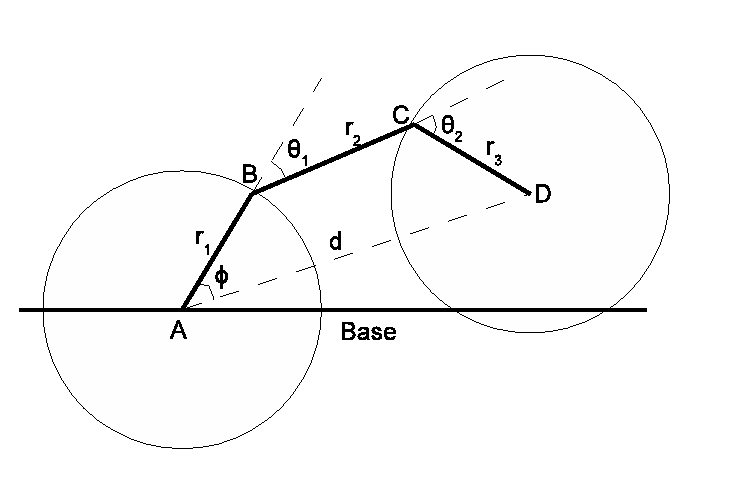
\includegraphics[scale=0.6]{images/two-circle.png}
\caption{Two Circle Algorithm}
\end{figure}

Following is a breif description of the algorithm :
 
  \begin{itemize}
  \item Rotate the base angle so that the robotic arm lies in the same vertical plane as the point we intend to reach.
  \item In this plane the arm looks as shown in Figure.
  \item We should find $\phi,\theta_1,\theta_2$ under the constraints are $AB=r_1,BC=r_2,CD=r_3,-\frac{\pi}{2}\le\phi,\theta_1,\theta_2\le\frac{\pi}{2},AD=d$.
  \item Observe that minimum value of $BC$ occurs when $\theta_1=\theta_2=0$ and maximum value of BC occurs when $\theta_1=\theta_2=\frac{\pi}{2}$(when BC is the direct common tangent for the two circles).
  \item So there will always exist a solution where $\theta_1=\theta_2=\theta$ and $0\le\phi,\theta\le\frac{\pi}{2}$.
  \item Moreover $BC$ will be a monotonic and continuous function of $\theta$, so we can do a binary search for the solution where $BC=r_2$.
  \item If $r_2>max BC$ then $\theta=\frac{\pi}{2}$ and if $r_2<min BC$ then $\theta=0$.
  \end{itemize}
  



\section{Testing Strategy}

\subsection{Modular Testing}
\begin{itemize}
\item Testing the API/library for real time serial port communication with the arm.\item Microsoft Visual Studio Professional 2010
\item Kinect for Windows SDK v1
\item .NET Framework 4.0 or higher
\item FT232 USB to Serial Converter (provided with the source)

\item Testing the skeletal data obtained using Kinect.
\item Testing the calculated angles and lengths required for the Two Circle Algorithm.
\item Testing the output of the Two Circle Algorithm.
\end{itemize}


\subsection{Combined Testing}
\begin{itemize} 
\item Testing the intuitiveness of the control by asking subjects to try to pick and place objects using the arm.
\item Testing the GUI for application, which is controls and connection various parameters.
\item Testing the effect of modifying various parameters of the algorithm and selecting the ones that give the best results.
\end{itemize}

\section{Code Reusability}
\begin{itemize}
\item Modules independent of each other, hence can be changed without changing others.
\item Developed an API/library for robotic arm control which future projects can use.
\item The algorithm for finding the arm angles also has wrappers which can  be reused.
\end{itemize}


\section{Requirements}
\subsection{Hardware}
\begin{itemize}
\item Microsoft Kinect Sensor
\item Dexter ER2 Heavy Duty Robotic Arm
\end{itemize}

\subsection{Software}
\begin{itemize}
\item Microsoft Visual Studio Professional 2010
\item Kinect for Windows SDK v1
\item .NET Framework 4.0 or higher
\item FT232 USB to Serial Converter (provided with the source)
\end{itemize}

\section{Usage Instructions}
\subsection{Installation}
The application is developed to run on the Windows platform only. Installation guide screencast is provided. The following dependencies need to be installed :
\begin{enumerate}
\item Kinect for Windows SDK v1
\item .NET Framework 4.0 or higher
\item FT232 USB to Serial Converter (provided with the source)
\end{enumerate}

Additionally, Microsoft Visual Studio Professional 2010 is required to modify/debug the source.

\subsection{Usage}
\begin{enumerate}
\item Connect the Kinect sensor to a power source and to the computer. 
\item Connect the Robotic Arm to a power source and to the computer. Press the Reset button on arm to reset the arm.
\item Run the executable 'KinectControlledRoboticArm.exe'.
\item Select the COM port to which the arm is connected from the drop-down menu.
\item Click on the Connect button.
\item Ask a friend to stand in front of the Kinect and make sure his skeletal frame is detected. This can be seen in the video feed from Kinect.
\item Change the elevation of the Kinect, if required, to make sure his arms are in the field of view of the Kinect even when his arms are completely stretched in any direction.
\item Click on the Start button.
\item The robotic arm can now be controlled using your right arm.
\item The gripper and wrist roll can be controlled using the left arm.
\item Click on the Stop button to stop controlling the arm.
\item Click on the Disconnect button to disconnect the arm from the computer.
\end{enumerate}

\section{Links}
\begin{itemize}
\item Project Home Page \\ \url{https://github.com/aayushssinghal/Kinect_Controlled_Robotic_Arm_group10_cs308_2012}
\item Hardware Setup Guide \\ \url{http://www.youtube.com/watch?v=o0-Mywjv-kc}
\item Software Setup and Usage Screencast\\ \url{http://www.youtube.com/watch?v=G3VrGSS2STc}
\end{itemize}

\section{References}
\begin{itemize}
\item Kinect for Windows SDK v1 : Resources and Documentation, Microsoft Corporation\\ \url{http://www.microsoft.com/en-us/kinectforwindows/develop/resources.aspx}
\item Kinect SDK v1 Quick Starts, Channel 9, MSDN\\ \url{http://channel9.msdn.com/Series/KinectQuickstart} 
\item Dexter ER2 Robotic Arm User Manual, Nex Robotics, Version 1.00, April 2011\\ \url{http://www.nex-robotics.com/products/robotic-arms-and-grippers/dexter-er-2-heavy-duty-robotic-arm-with-controller-and-accessories.html}
\item AVR AtMega2560 Programming Manual, Atmel, May 2011 \\ \url{http://www.atmel.com/Images/doc2549.pdf}
\end{itemize}


\end{document}

